\documentclass{llncs}

\usepackage[T1]{fontenc}
\usepackage[utf8]{inputenc}
\usepackage{amsmath,amssymb}
\usepackage{booktabs}
\usepackage{array}
\usepackage{listings}
\usepackage{hyperref}
\usepackage{microtype}
\usepackage{float}
\usepackage{mdframed}
\usepackage{graphicx}
\usepackage{etoolbox}
\graphicspath{{figs/}}

\emergencystretch=1em
\def\UrlBreaks{\do\/\do\-\do\_\do.}

% ── Vertical spacing tightening ───────────────────────────────────────────────
\setlength{\parskip}{0pt}
\setlength{\tabcolsep}{4pt}
\renewcommand{\arraystretch}{0.92}

\setlength{\abovedisplayskip}{5pt plus 1pt minus 1pt}
\setlength{\belowdisplayskip}{5pt plus 1pt minus 1pt}
\setlength{\abovedisplayshortskip}{3pt}
\setlength{\belowdisplayshortskip}{3pt}

\setlength{\textfloatsep}{8pt plus 2pt minus 2pt}
\setlength{\floatsep}{6pt plus 2pt minus 2pt}
\setlength{\intextsep}{6pt plus 2pt minus 2pt}

\makeatletter
\patchcmd{\@begintheorem}{\trivlist}%
  {\setlength{\topsep}{3pt}\setlength{\partopsep}{0pt}\trivlist}%
  {}{}
\makeatother

\makeatletter
\renewcommand\section{\@startsection{section}{1}{\z@}%
  {-1.2ex \@plus -0.2ex \@minus -.1ex}%
  {0.6ex \@plus .1ex}%
  {\normalfont\large\bfseries}}
\renewcommand\subsection{\@startsection{subsection}{2}{\z@}%
  {-1.0ex \@plus -0.2ex \@minus -.1ex}%
  {0.4ex \@plus .1ex}%
  {\normalfont\normalsize\bfseries}}
\makeatother

\hypersetup{colorlinks=true,linkcolor=black,citecolor=black,urlcolor=black}

\lstset{basicstyle=\ttfamily\small,frame=single,breaklines=true,
        aboveskip=0.6em,belowskip=0.6em}

\spnewtheorem{observation}[theorem]{Observation}{\bfseries}{\itshape}
\spnewtheorem{principle}[theorem]{Principle}{\bfseries}{\itshape}

\DeclareMathOperator{\dist}{dist}
\newcommand{\ecollapse}{\varepsilon_{\mathrm{c}}}
\newcommand{\emeta}{\varepsilon_{\mathrm{m}}}
\newcommand{\st}[1]{\textup{\textsc{#1}}}

\newmdenv[leftmargin=0pt,rightmargin=0pt,
          innerleftmargin=10pt,innerrightmargin=10pt,
          innertopmargin=6pt,innerbottommargin=6pt,
          linewidth=0.8pt]{tracebox}

% Draft version marker: v10 -- targeted expansion after confirming references do not count toward the 16-page body limit
\begin{document}

\title{Structural Fatigue and Metastable Closure in Runtime Monitoring}
\author{Duston Moore}
\institute{Independent Researcher \\ \email{dhwcmoore@gmail.com}}
\maketitle

\begin{abstract}
Operational closure does not imply structural safety: admissibility
degradation accumulates historically and is not reset on reclosure. This
condition is metastable closure. We extend admissibility with a temporal guard, timely admissibility, which fails when the remaining rupture horizon is no greater than the monitor's admissibility lag. STAK-PSAL detects metastable closure via $\mathcal{F}_n$,
a cumulative fatigue metric invisible to instantaneous monitors. A formal
layer (machine-checked Coq proofs of structural separation and threshold contraction) grounds an operational
$\varepsilon$-admissible OCaml monitor. Metastably closed runs exhibit
13.8--14.9$\times$ higher $\mathcal{F}_n$ than stably recovered runs
with identical runtime status; in the evaluated model family, the
\st{critical} forecast yields zero false negatives across 2,159 ruptured
runs with mean lead time 11.6 to 13.7 steps.
\end{abstract}

% ── 1. Introduction ───────────────────────────────────────────────────────────
\section{Runtime Preservation of Safety-Relevant Distinguishability}
\label{sec:problem}

A runtime system may remain operationally closed while already possessing
a bounded rupture horizon. A runtime monitor may certify closure even
when the system has accumulated admissibility fatigue that renders future
collapse substantially more likely. This danger is not visible in
instantaneous outputs or anomaly scores: two systems may present
identical runtime observations while differing radically in structural
fatigue and future rupture trajectory.

We introduce STAK-PSAL (Structural Tension and Admissibility with a
Parallel Structural Assurance Layer), a runtime monitoring architecture
for detecting metastable closure under cumulative admissibility fatigue.
The intended domain is continuous or quasi-continuous degradation in
cyber-physical observation maps. This matters: the argument does not
begin from a general theory of intelligent systems, nor from discrete
symbol generation, but from a setting in which a safety-relevant
separation margin can narrow smoothly while ordinary outputs remain
nominal. The scope restriction is methodological rather than incidental;
it is what allows fatigue, horizon, and enrichment to be treated as
runtime quantities rather than as post hoc explanations of failure.

\begin{table}[tbp]
\centering
\caption{Identical runtime snapshots; divergent structural states
  (empirical means, 7,800 runs)}
\label{tab:hidden}
\footnotesize
\begin{tabular}{@{}p{0.28\linewidth}p{0.31\linewidth}p{0.31\linewidth}@{}}
\toprule
\textbf{Property} & \textbf{Stable recovery (R3)} & \textbf{Metastable closure (R2)} \\
\midrule
Current status                   & \st{closed} & \st{closed} \\
Instantaneous $d_t$              & $0.43$      & $0.44$ \\
Output anomaly                   & nominal     & nominal \\
Prior \st{meta\_review} episodes & $0$         & ${\geq}1$ \\
Mean $\mathcal{F}_n$             & $0.165$     & $2.462$ \\
Future rupture rate              & $0\%$       & $100\%$ \\
\bottomrule
\end{tabular}
\end{table}

Table~\ref{tab:hidden} is not hypothetical: these are empirically
observed properties across 7,800 evaluated runs; a monitor classifying
by current status or instantaneous $d_t$ cannot distinguish them, but
$\mathcal{F}_n$ can (Section~\ref{sec:experiments}).
Current admissibility is instantaneous: it classifies the present
reduction. Structural fatigue is historical: it records the cumulative
cost required to preserve admissibility across prior destabilisations.

A cyber-physical system reduces state $\mathcal{X} = \mathbb{R}^n$ to
observations $\mathcal{O} = \mathbb{R}^m$ via $M_t$; safety requires
$M_t$ to preserve all safety-relevant distinctions. Static verification
certifies $M_0$ and says nothing about $M_t$ for $t > 0$. Degradation
collapses safety-distinct states into identical observations while every
individual output remains in-distribution. Anomaly detectors miss this;
output monitors detect deviations in $M_t(x)$ but not in
$\dist(M_t(x), M_t(y))$.

\begin{example}[Industrial pressure monitor]
\label{ex:valve}
A 64-dimensional industrial sensor vector spans pressure, temperature,
flow, and vibration modalities. The safety function $\Phi(z) = \st{estop}$
iff $z_0 > 0.70$. Two systems operate under identical parameters
($\delta = 0.020$, $b = 0.10$): one achieves stable recovery (R3) and
one re-enters the warning band after apparent reclosure, subsequently
rupturing (R2). Both inputs remain in-distribution as $W_t$ degrades
(Figure~\ref{fig:blindspot}). At the moment of reclosure both systems
present identical runtime status; only $\mathcal{F}_n$ distinguishes
them.
\end{example}

\begin{figure}[tbp]
\centering
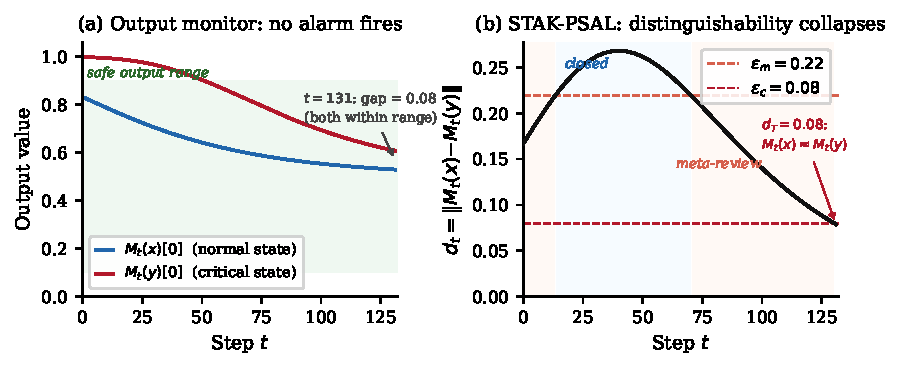
\includegraphics[width=0.70\linewidth]{fig_blindspot.pdf}
\caption{Statistical normality may coexist with admissibility collapse.
Output monitoring remains silent while $d_t$ approaches $\ecollapse$.}
\label{fig:blindspot}
\end{figure}

The principal contribution is the identification, formal
characterisation, and operational detection of \emph{metastable closure}: a run classified as operationally
closed while carrying a bounded rupture horizon. Closure excludes present rupture, but it does not exclude horizon collapse.
\emph{First}, structural divergence under operational equivalence is machine-checked in the
metastable recovery semantics (Section~\ref{sec:mrp}). \emph{Second},
a bridge from strict to $\varepsilon$-admissibility: under geometric
contraction, threshold crossing from $\varepsilon$ to any
$\varepsilon' < \varepsilon$ is guaranteed in bounded steps
(Section~\ref{sec:opapprox}). \emph{Third}, we introduce timely admissibility and Horizon Debt to formalise the collapse of the repair envelope when the remaining horizon falls below the admissibility lag. \emph{Fourth}, $\mathcal{F}_n$ is
validated as a predictive estimator: in the evaluated model family,
\st{critical} has zero false negatives and mean lead time 11.6 to 13.7
steps across 7,800 runs (Sections~\ref{sec:monitor}--\ref{sec:experiments}).
\emph{Fifth}, the enrichment mechanism is identified as a security boundary:
the same elasticity that permits recovery can be exhausted by repeated
bounded perturbations, producing adversarial elasticity inversion
(Sections~\ref{sec:estimators} and~\ref{sec:security}). The monitor is
scoped to continuous degradation; applicability beyond this regime is an
open boundary (Section~\ref{sec:limits}). Unlike anomaly, drift, and
uncertainty monitors, STAK-PSAL monitors preservation of safety-relevant
distinguishability rather than unusual traces, distributional shift, or
confidence loss.
The architecture is also deployment-conservative: STAK-PSAL may run as a read-only sidecar with full observational access but no actuation authority.

% ── 2. Failure of Static Admissibility ────────────────────────────────────────
\section{Failure of Static Admissibility}
\label{sec:failure}

\subsection{Deployment Architecture Assumptions}
\label{sec:deploy-assumptions}

STAK-PSAL presumes white-box access to $M_t$. It also presumes an
observational enrichment pathway: either mutable access to the weight
matrix or an equivalent runtime resource such as secondary sensing,
adaptive sampling, or operator escalation.

\paragraph{Read-only sidecar deployment.}
STAK-PSAL is intended to be deployable outside the authority-bearing control loop. In its conservative industrial configuration, the monitor runs as a read-only sidecar with mirrored access to sensor streams, controller traces, actuator-command logs, and derived state estimates, but with no authority to issue commands, modify thresholds, reset controller state, or actuate the plant. Its outputs are advisory and evidential: it emits monitor states, fatigue measurements, meta-review warnings, and rupture certificates. The plant controller, safety interlock, or human operator remains the only authority capable of intervention. This separation is important because the monitor is asked to judge the structural reliability of an observational reduction, not to replace the controller whose reductions it audits. Initial deployment can therefore proceed in shadow mode: STAK-PSAL observes the same operational history as the controller, records cumulative fatigue and enrichment use, and produces signed evidence without introducing a new actuation pathway.

\subsection{The Degradation Trajectory}

Under the weight update $W_{t+1} = (1-\delta)\,W_t$, the separation
$d_t$ decreases monotonically toward 0 (Figure~\ref{fig:blindspot}b).
At $\delta = 0.020$, rupture occurs at step 114; the horizon is a function
of degradation rate and initial margin, neither readable from the initial
admissibility certificate. Verification of $M_0$ does not certify $M_{71}$.

\subsection{Enrichment Triage as Observational Resolution Enhancement}

Enrichment is the operational escalation triggered on entry to the
warning band. In the demonstrator it is realised as a targeted weight
boost: on detecting that $d_t$ has fallen into
$(\ecollapse, \emeta]$, the dimension $j^* = \arg\max_j |x_j - y_j|$
in row 0 of $W_t$ receives a one-time additive boost $b > 0$.

The weight-boost is one representative observational-resolution
enhancement. In trusted deployments, enrichment may modify $W_t$ or raise
sampling rate; in certified or adversarial deployments, it may activate
secondary sensors, corroborating modalities, or operator escalation. The
theory requires only an estimated gain $g_m$ and loss term $\ell_m\Delta_t$.
The projected post-intervention margin $d^{\mathrm{post}}_m$ for mechanism $m$ is:
\[
d^{\mathrm{post}}_m = d_t - \ell_m \Delta_t + q_m g_m .
\]

\[
\mathcal{E}^{\mathrm{res}}_m(t) = q_m g_m - \ell_m \Delta_t .
\]

A mechanism is survival-viable if $d^{\mathrm{post}}_m > \ecollapse$, reclosure-viable if $d^{\mathrm{post}}_m > \emeta$, and durably viable if it restores $d^{\mathrm{post}}_m > \emeta$ while leaving post-intervention horizon greater than the admissibility lag.

\paragraph{Enrichment budget.}
Enrichment fires once per \st{meta\_review} entry; the boosted weight
erodes at rate $\delta$, injecting a margin that subsequently decays.
The operational layer therefore has finite enrichment capacity: repeated
escalation consumes observational elasticity and may itself induce
metastable behaviour. A reclosed system will reach the warning threshold
again sooner than one never destabilised. This budget asymmetry is the
operational mechanism behind the MRP (Section~\ref{sec:mrp}); adversarial
implications are in Section~\ref{sec:security}.

The finite budget creates two dual threats. Horizon Debt occurs when the
remaining rupture horizon is no greater than the admissibility lag, so
waiting is no longer certified even though rupture has not yet occurred.
Adversarial elasticity inversion occurs when repeated boundary-near
perturbations consume recovery elasticity without corresponding physical
degradation. The first is a timing failure; the second is a provenance
failure. Both are invisible to a monitor that observes only current
closure status.

% ── 3. Admissibility Definitions ──────────────────────────────────────────────
\section{Admissibility Definitions}
\label{sec:defs}

Let $\mathcal{X} = \mathbb{R}^n$, $\mathcal{O} = \mathbb{R}^m$, $m \ll n$.
Let $\mathcal{A}$ be a finite action set and $\Phi : \mathcal{X} \to
\mathcal{A}$ a safety function.

\begin{definition}[Reduction operator]
\label{def:reduction}
$M_t : \mathcal{X} \to \mathcal{O}$; in the demonstrator $M_t(z) =
\sigma(W_t \cdot z)$ for $W_t \in \mathbb{R}^{2 \times 64}$.
\end{definition}
\begin{definition}[Admissibility (strict)]
\label{def:admissibility}
$M_t$ is admissible w.r.t.\ $\Phi$ if $M_t(x) = M_t(y) \Rightarrow
\Phi(x) = \Phi(y)$.
\end{definition}
\begin{definition}[$\varepsilon$-admissibility]
\label{def:eps}
$M_t$ is $\varepsilon$-admissible if
\[ \Phi(x) \neq \Phi(y) \;\Rightarrow\; \dist(M_t(x), M_t(y)) > \varepsilon. \]
Definition~\ref{def:admissibility} is the $\varepsilon \to 0$ limit;
the formal layer reasons over Definition~\ref{def:admissibility}, the
operational layer uses Definition~\ref{def:eps} with $\varepsilon =
\ecollapse$. The bridge is in Section~\ref{sec:opapprox}.
\end{definition}

\begin{definition}[Boundary, rupture, closure]
\label{def:boundary}\label{def:rupture}\label{def:closure}
A \emph{boundary} is $B \subseteq \mathcal{X}$ with $x \in B, y \notin
B \Rightarrow \Phi(x) \neq \Phi(y)$; $M_t$ is \emph{boundary-preserving}
if $x \in B, y \notin B \Rightarrow \dist(M_t(x), M_t(y)) > \ecollapse$
(in Example~\ref{ex:valve}, $B = \{z \mid z_0 > 0.70\}$). A
\emph{rupture} at $t^*$ is a pair $(x, y)$ with $\Phi(x) \neq \Phi(y)$
and $\dist(M_{t^*}(x), M_{t^*}(y)) \leq \ecollapse$; no correct safety
decision is recoverable from $M_{t^*}(x)$ alone. The system is
\emph{closed} at $t$ if $M_t$ is $\varepsilon$-admissible and
$\dist(M_{t+1}, M_t) \leq \eta$ for $\eta > 0$ (current admissibility
plus local stability).
\end{definition}

\begin{definition}[Rupture certificate]
\label{def:cert}
A \emph{rupture certificate} is a triple $(x, y, t^*)$ such that $(x,y)$
is a rupture at $t^*$, with the following three witnesses. The
\emph{logical witness} establishes
$\dist(M_{t^*}(x), M_{t^*}(y)) \leq \ecollapse$ and
$\Phi(x) \neq \Phi(y)$. The \emph{operational witness} records the
divergent actions with their physical interpretations. The
\emph{instability witness} records the sequence of boundary
revisions, oscillation count, and peak tension preceding $t^*$.
\end{definition}

\begin{definition}[Runtime estimator]
\label{def:estimator}
A \emph{runtime estimator} is a computable function
$\mathcal{E} : \mathit{States} \times \mathit{History} \to \mathbb{R}$
that tracks a structural property; it signals proximity to rupture
without certifying it.
\end{definition}

\paragraph{Horizon debt certificate.}
A \texttt{HorizonDebtCertificate} is emitted before hard rupture when \(h_t\leq L_t\). It records that the system is not yet ruptured, but is no longer safe to wait. In the illustrative run, the certificate fires at \(t=49\) with \(d_t=0.0915\), \(\epsilon_c=0.08\), \(h_t=2\), and \(L_t=2\). Adaptive sampling is survival-viable: it keeps \(d_t\) above \(\epsilon_c\), but does not restore \(d_t>\epsilon_m\). Hard rupture follows at \(t=53\), showing that the certificate identified a narrowed repair envelope, not an already ruptured state.

Let \(V_m(t)\in\{0,1,2,3\}\) denote the viability rank of mechanism \(m\): not viable, survival-viable, reclosure-viable, or durably viable. The one-step opportunity cost is
\[
\mathrm{OppCost}_m(t)=\max(0,V_m(t-1)-V_m(t)).
\]
It records the collapse of the repair envelope, not the collapse of the observation margin.

In RV terms, $\varepsilon$-admissibility is a runtime-checkable
separation invariant; rupture is monitor indistinguishability failure;
metastable closure is confirmed recovery with accumulated admissibility
deficit; and the \st{critical} forecast is an anticipatory violation signal.

% ── 4. The Three-State Monitor ────────────────────────────────────────────────
\section{The Three-State Monitor}
\label{sec:monitor}

{\sloppy\noindent\textbf{Monitor contract.}
The monitor inputs are $(d_t,\allowbreak\, \mathit{status}_{t-1},\allowbreak\, W_t)$;
the output is $(\mathit{status}_t,\, \mathit{cert})$, with
$\mathit{cert}$ populated iff $\mathit{status}_t = \st{hard\_rupture}$.
The invariant is: \st{closed} status implies $M_t$ is
$\varepsilon$-admissible (Theorem~\ref{thm:coq}, (T4)). Escalation from
\st{closed} occurs on $d_t \in (\ecollapse, \emeta]$; escalation from
\st{meta\_review} occurs on $d_t \leq \ecollapse$. The \st{critical}
signal precedes every confirmed \st{hard\_rupture} (zero false negatives,
7,800 runs) with mean lead time 11.6 to 13.7 steps.\par}

The monitor maintains a weight matrix $W_t \in \mathbb{R}^{2 \times 64}$
and a fixed critical pair $(x, y)$ with $\Phi(x) \neq \Phi(y)$.
The reduction is $M_t(z) = \sigma(W_t \cdot z)$.
On each step, weights decay: $W_{t+1} = (1-\delta)\,W_t$.
On \st{closed}$\to$\st{meta\_review} transition, enrichment fires
once: the dimension $j^* = \arg\max_j |x_j - y_j|$ in row 0 of $W_t$
receives a one-time boost $b > 0$.

\st{closed} ($d_t > \emeta$): $\varepsilon$-admissible, no action.
\st{meta\_review} ($\ecollapse < d_t \leq \emeta$): admissible but
degrading; enrichment fires once on entry, autonomous execution
restricted; reclosure if $b \geq b_{\mathrm{crit}}$, otherwise $d_t$
falls to rupture. \st{hard\_rupture} ($d_t \leq \ecollapse$):
admissibility failed; certificate emitted (Definition~\ref{def:cert}),
monitoring halts. Thresholds: $\ecollapse = 0.08$, $\emeta = 0.22$
($d_0 \approx 0.72$).

\subsection{State Transition Semantics}

Table~\ref{tab:transitions} gives the complete state machine.

\begin{table}[tbp]
\centering
\caption{State transitions (C = \st{closed}, M = \st{meta\_review},
  H = \st{hard\_rupture})}
\label{tab:transitions}
\small
\begin{tabular}{llll}
\toprule
\textbf{From} & \textbf{Condition on $d_t$} & \textbf{To} & \textbf{Action} \\
\midrule
C & $d_t > \emeta$             & C & none \\
C & $\ecollapse < d_t \leq \emeta$ & M & Enrichment fires on $j^*$ \\
C & $d_t \leq \ecollapse$         & H & Certificate emitted; halt \\
M & $d_t > \emeta$             & C & Reclosure recorded \\
M & $\ecollapse < d_t \leq \emeta$ & M & Estimators updated; no enrichment \\
M & $d_t \leq \ecollapse$         & H & Certificate emitted; halt \\
H & all                        & H & Terminal state \\
\bottomrule
\end{tabular}
\end{table}

\subsection{The Enrichment/Degradation Balance and $b_{\mathrm{crit}}$}

The critical boost value $b_{\mathrm{crit}}(\delta)$ is the minimal $b$
for which stable-recovery outcomes (reclosure without subsequent rupture)
constitute a majority at 100 seeds. Experimentally, $b_{\mathrm{crit}}$
scales linearly:

\begin{equation}
  b_{\mathrm{crit}}(\delta) \approx 10\delta
  \label{eq:bcrit}
\end{equation}

Valid across $\delta \in \{0.010, \ldots, 0.030\}$; not extrapolated
beyond the evaluated regime.

\subsection{Formal Invariants and Their Operational Role}
\label{sec:coq}

The following invariants are machine-checked over
Definition~\ref{def:admissibility}. They constrain the structural
relations between admissibility, boundary preservation, closure, and
the rupture certificate; the operational monitor instantiates these as
$\varepsilon$-regime approximations.

\begin{theorem}[Coq invariants]
\label{thm:coq}
\label{thm:anr}\label{lem:cir}\label{thm:cer}
Over Definitions~\ref{def:admissibility}--\ref{def:cert} the following
hold:
\begin{align*}
\textrm{(T1)\;}\texttt{admissible\_not\_ruptured}:\;
    &\mathit{Admissible} \Rightarrow \neg\,\mathit{Rupture} \\
\textrm{(T2)\;}\texttt{boundary\_preservation}:\;
    &\mathit{BoundaryPreserved} \Rightarrow \mathit{Admissible} \\
\textrm{(T3)\;}\texttt{certificate\_implies\_rupture}:\;
    &\mathit{RuptureCertificate} \Rightarrow \mathit{Rupture} \\
\textrm{(T4)\;}\texttt{closure\_excludes\_rupture}:\;
    &\mathit{Closure} \Rightarrow \neg\,\exists\,\mathit{RuptureCertificate} \\
\textrm{(T5)\;}\texttt{rupture\_implies\_violation}:\;
    &\mathit{Rupture} \Rightarrow \neg\,\mathit{BoundaryPreserved}
\end{align*}
A direct corollary of \textrm{(T3)} is $\mathit{RuptureCertificate}
\Rightarrow \neg\,\mathit{Admissible}$.
\end{theorem}

\subsection{Operational Approximation and $\varepsilon$-Admissibility}
\label{sec:opapprox}

The formal theorems and operational monitor occupy different
mathematical regimes (Table~\ref{tab:layers}): theorems over strict
admissibility (Definition~\ref{def:admissibility}), the monitor over
$\varepsilon$-admissibility (Definition~\ref{def:eps}).

\begin{table}[tbp]
\centering
\caption{Two layers of the monitor architecture}
\label{tab:layers}
\small
\begin{tabular}{ll}
\toprule
\textbf{Formal layer} & \textbf{Operational layer} \\
\midrule
Strict equality $M(x) = M(y)$       & $\varepsilon$ margin $\dist(M(x),M(y)) > \varepsilon$ \\
Theorem space                       & Continuous runtime monitoring \\
Exact admissibility                 & Approximate admissibility \\
Coq proofs                          & Empirical OCaml prototype \\
Boundary conditions for the monitor & Step-by-step runtime decisions \\
\bottomrule
\end{tabular}
\end{table}

The machine-checked semantic hierarchy fixes structural relations at the
strict-equality limit; the OCaml monitor approximates these at finite
$\varepsilon$. The machine-checked existential bridge
(\texttt{formal/\allowbreak{}threshold\_bridge.v}) connects them: under geometric
contraction, if $d_t \leq \varepsilon$, then for any $\varepsilon' \in
(0, \varepsilon)$ there exists $k$ such that $d_{t+k} \leq \varepsilon'$.
The explicit logarithmic ceiling bound on the horizon $T$ stated below
is a quantitative refinement of that machine-checked existential.

\begin{lemma}[Operational rupture bound]
\label{lem:opbound}
Let $M_t(z) = \sigma(W_t z)$ with $W_{t+1} = (1-\delta) W_t$ and
$\sigma$ Lipschitz with constant $L_\sigma$. If $d_t = \dist(M_t(x),
M_t(y)) \leq \varepsilon$, then for any $\varepsilon' \in (0,
\varepsilon)$ the horizon $T = t' - t$ at which $d_{t'} \leq
\varepsilon'$ satisfies
\[
  T \;\leq\;
    \left\lceil
      \frac{\log(\varepsilon / \varepsilon')}{\log(1 / (1-\delta))}
    \right\rceil
    \;\approx\;
    \left\lceil
      \frac{1}{\delta}\,\log\!\frac{\varepsilon}{\varepsilon'}
    \right\rceil .
\]
The operational regime at threshold $\varepsilon$ collapses into the
regime at any $\varepsilon' < \varepsilon$ in bounded, explicitly
computable time; the strict regime $d_{t'} \to 0$ is the asymptotic
limit.
\end{lemma}

\begin{proof}[Sketch]
Multiplicative decay gives $W_{t'}=(1-\delta)^T W_t$ for $T=t'-t$.
For a fixed critical pair, the pre-activation separation therefore scales
as $(1-\delta)^T\|W_t(x-y)\|$. Since $\sigma$ is Lipschitz, there is a
constant $C$ determined by $L_\sigma$ and the chosen projection norm such
that $d_{t'}\leq C(1-\delta)^T d_t$. Absorbing $C$ into the operational
choice of threshold, or equivalently replacing $\varepsilon'$ by
$\varepsilon'/C$, reduces the crossing condition to
$(1-\delta)^T\varepsilon\leq\varepsilon'$. Solving for $T$ gives the
stated ceiling bound. The Lipschitz constant is therefore not an
additional empirical assumption about the run; it is the regularity
condition that prevents the strict-to-$\varepsilon$ bridge from becoming
an uncontrolled discontinuity.
\end{proof}

The machine-checked existential bridge guarantees threshold crossing in
bounded steps; the explicit logarithmic ceiling bound is the quantitative
refinement isolating the precise horizon. The role of the bound is to
make the operational approximation measurable: the strict Coq layer gives
the limiting structural relation, while the OCaml monitor tracks the
finite margin at which that relation becomes actionable. The approximation
is therefore a controlled slope, not a cliff between proof and prototype.

\paragraph{Timely admissibility.}
Strict admissibility is instantaneous. It says that the current observation map preserves the distinctions required by \(\Phi\). Runtime assurance requires that this preservation remain actionable before the rupture horizon closes. Let \(h_t\) be the estimated remaining rupture horizon and \(L_t\) the admissibility lag of the monitor. Define
\[
\mathrm{TimelyAdmissible}(M_t,\Phi,h_t,L_t)
:=
\mathrm{Admissible}(M_t,\Phi)\wedge L_t<h_t.
\]
Horizon Debt is the condition \(h_t\leq L_t\). It does not assert rupture. It asserts loss of safe waiting:
\[
\mathtt{META\_REVIEW}_t \wedge h_t\leq L_t
\Rightarrow \neg \mathrm{SafeToWait}_t .
\]

\subsection{Bounding the Operational Approximation}
\label{sec:opbound-empirical}

As $\delta$ increases, the predictive horizon shrinks:
$T \approx (1/\delta)\log(\varepsilon/\varepsilon')$
(Lemma~\ref{lem:opbound}). The stochastic sweep
(Section~\ref{sec:stoch-sweep}) validates this bound empirically. At
$\delta = 0.015$, mean \st{critical} lead time is 16.8 steps; at $\delta
= 0.030$ it collapses to 9.4 steps, with a minimum of 1 step in the
most rapid degradation cases. This matches the asymptotic expectation:
at $\delta = 0.030$ the bound $T = (1/0.030)\log(\ecollapse/\varepsilon')
\approx 33$ steps to strict collapse is consistent with the observed
compressed lead-time distribution.

% ── 5. Predictive Instability Estimation ──────────────────────────────────────
\section{Predictive Instability Estimation}
\label{sec:estimators}

The four signals below are runtime estimators
(Definition~\ref{def:estimator}), each active several steps before
$d_t$ crosses $\ecollapse$. Of these, $\mathcal{F}_n$ is
architecturally primary: the only signal that accumulates across
episodes rather than evaluating instantaneous state. Instantaneous
admissibility cannot distinguish metastable closure from stable
recovery; $\mathcal{F}_n$ operationalises cumulative structural
degradation invisible to state-local monitoring.

\textbf{Tension slope.}
Let $T_t$ be the tension score (weighted EMA of the separation deficit).
\begin{equation}
  \dot{T}_t = \alpha_s (T_t - T_{t-1}) + (1-\alpha_s)\dot{T}_{t-1},
  \quad \alpha_s = 0.25
  \label{eq:slope}
\end{equation}

\textbf{Separation EMA.}
\begin{equation}
  \bar{d}_t = \alpha_d\, d_t + (1-\alpha_d)\,\bar{d}_{t-1},
  \quad d_t = \dist(M_t(x), M_t(y)),
  \quad \alpha_d = 0.10
  \label{eq:sep-ema}
\end{equation}

\textbf{Rupture pressure.}
\begin{equation}
  R_t = \frac{1}{d_t + \varepsilon_0}, \quad \varepsilon_0 = 0.001
  \label{eq:rp}
\end{equation}

\textbf{Recovery elasticity.}
Let $T_{\mathrm{entry}}$ be the tension at \st{meta\_review} entry and
$\Delta t$ the steps elapsed since enrichment fired.
\begin{equation}
  E_r^{(t)} = \frac{T_{\mathrm{entry}} - T_t}{\Delta t}
  \label{eq:elast}
\end{equation}
$E_r^{(t)} > 0$ indicates recovery in progress; $E_r^{(t)} < 0$
indicates degradation outpacing enrichment. Defined only for
$\mathtt{steps\_in\_meta} > 2$.

\begin{definition}[Adversarial elasticity inversion]
\label{def:aei}
An \emph{adversarial elasticity inversion} occurs when $E_r^{(t)} < 0$
and $|\Delta P_t| \leq \eta_P$ over a sustained \st{meta\_review}
interval, where $P_t$ denotes the monitored physical degradation proxy
and $\eta_P$ is the expected physical drift bound. In this case, loss of
recovery elasticity is not explained by the monitored physical
degradation proxy. The remaining explanation is exhaustion of the
enrichment pathway, which may be benign or adversarial depending on
provenance.
\end{definition}

The compound condition $E_r^{(t)} < 0$ with bounded $|\Delta P_t|$ and
repeated \st{meta\_review} entry constitutes a bounded rupture claim of
potentially adversarial origin (Section~\ref{sec:security}). Note that
negative elasticity alone is necessary but not sufficient for rupture:
100\% of R2 runs exhibit it, but so do 20\% of R3 runs
(Table~\ref{tab:fatigue}). The adversarial interpretation requires the
additional condition of bounded physical drift.

\textbf{Cumulative fatigue.}
\begin{equation}
  \mathcal{F}_{t+1} = \mathcal{F}_t
    + \lambda_1 |\Delta T_t|
    + \lambda_2 \max(0, -E_r^{(t)})
    + \lambda_3 \max(0, R_t - R_0)
  \label{eq:fatigue}
\end{equation}
Accumulated during \st{meta\_review} steps only
($\lambda_1 = 1.0$, $\lambda_2 = 0.1$, $\lambda_3 = 0.01$,
$R_0 = 5.0$); not reset on reclosure. \(\mathcal{F}_n\) is not an anomaly magnitude. It is a memory variable
that records the cumulative enrichment expenditure required to preserve
runtime admissibility.

\begin{definition}[\st{critical} forecast]
\label{def:critical}
The system is in \st{critical} state at $t$ when:
\begin{equation}
  \dot{T}_t > \theta_s
  \;\land\;
  R_t > R_c
  \;\land\;
  E_r^{(t)} < E_w
  \;\land\;
  \mathtt{steps\_in\_meta} > 2
  \label{eq:critical}
\end{equation}
where $\theta_s = 0.002$, $R_c = 10.0$, $E_w = 0.005$ (calibrated on
the 13-run deterministic sweep; stochastic and benchmark results are
out-of-calibration evaluations). \st{critical} signals closing intervention
window; a system satisfying \eqref{eq:critical} may still recover at higher
boost levels.
\end{definition}

% ── 6. OCaml/Coq Implementation ───────────────────────────────────────────────
\section{OCaml/Coq Implementation}
\label{sec:impl}

{\sloppy
The monitor is implemented in OCaml~4.14 and Coq~8.18. The OCaml modules separate
core types (\texttt{types.ml}), reduction/degradation/enrichment
(\texttt{lnp.ml}), admissibility checks (\texttt{admissibility.ml}),
estimators (\texttt{tension.ml}), state transitions and fatigue
(\texttt{machine.ml}), instability classification
(\texttt{instability.ml}), certificate emission (\texttt{certificate.ml}),
and the four-modality benchmark (\texttt{scenario.ml}). The Coq layer
contains the invariant file \texttt{formal/stak\_psal.v}, contraction
core \texttt{formal/contraction\_core.v}, threshold bridge
\texttt{formal/threshold\_bridge.v}, and metastable recovery semantics
\texttt{formal/metastable\_recovery.v}.\par}

Each step computes $(d_t,\bar{d}_t,\dot{T}_t,R_t,E_r^{(t)})$ followed
by state transition and optional certificate emission. Enrichment fires
once per \st{closed}$\to$\st{meta\_review} transition; the certificate
builder populates all three witnesses of Definition~\ref{def:cert} and
serialises to JSON.

% ── 7. Experimental Evaluation ────────────────────────────────────────────────
\section{Experimental Evaluation}
\label{sec:experiments}

The experiments establish two claims: (1) metastably closed runs are
distinguishable from stably recovered runs by $\mathcal{F}_n$ alone;
(2) \st{critical} provides advance warning before confirmed collapse.
All three settings share the same parameters:
$\ecollapse = 0.08$, $\emeta = 0.22$, $W_0[0][0] = 5.0$, $n = 64$,
$m = 2$.

\subsection{Representative trace}
\label{sec:trace}

A representative R2 run ($\delta = 0.020$, $b = 0.10$, seed 42)
demonstrates the principle: the two \st{closed} intervals are
indistinguishable under instantaneous $d_t$ but separable by cumulative
fatigue $\mathcal{F}_n$ (2.94 at rupture, $17.8\times$ the R3 mean);
\st{critical} fires 12 steps before. Representative metastable trajectories exhibit:
(i)~temporary reclosure, (ii)~renewed decline in $d_t$,
(iii)~negative elasticity, and (iv)~cumulative fatigue accumulation
despite apparent recovery.

Figure~\ref{fig:comparison} shows a paired R3/R2 run: both reclose at
$t = 61$ with identical $d_t$ and status; R2 re-enters
\st{meta\_review} and ruptures at $t = 121$, \st{critical} firing 11
steps before, with structural divergence already visible in
$\mathcal{F}_n$.

\begin{figure}[tbp]
\centering
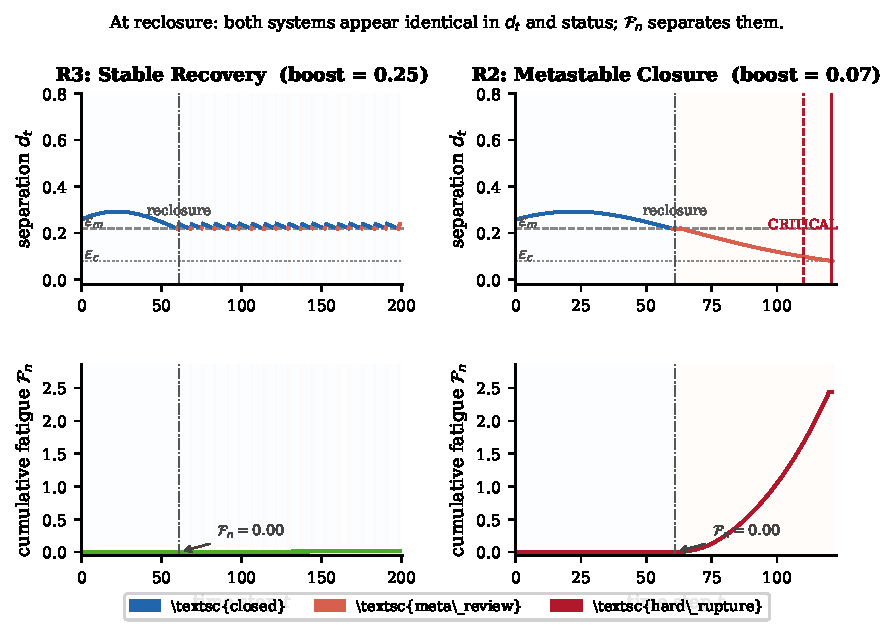
\includegraphics[width=0.86\linewidth]{fig4_comparison.pdf}
\caption{R3 (stable recovery, left) and R2 (metastable closure, right) with
  the same seed and identical parameters except boost (0.25 vs.\ 0.05).
  Both reclose at $t = 61$; $d_t$ and status are indistinguishable at that
  moment. $\mathcal{F}_n$ (bottom row) separates them: R2 carries
  substantially higher cumulative fatigue into its second episode.}
\label{fig:comparison}
\end{figure}

\subsection{Deterministic bifurcation sweep}
\label{sec:det-sweep}

Single noise-free input pair, $\delta = 0.020$,
$b \in \{0.00, 0.05, \ldots, 0.60\}$ (13 runs), $T = 200$ steps. Three
regimes appear at $b_{\mathrm{crit}} = 0.20$: R1 ($b=0$, rupture step
114), R2 ($b \in [0.05, 0.15]$, reclosed once then ruptured at steps
118 to 187), R3 ($b \geq 0.20$, stable). \st{critical} fires iff the
run ruptures: 0 FP, 0 FN, mean lead time 11.5 steps (range 10 to 14) on
13 runs; confirmed at scale in Section~\ref{sec:stoch-sweep}.

\subsection{Stochastic sweep}
\label{sec:stoch-sweep}

100 seeds per cell, 13 boost values, five degradation rates
$\delta$ from $0.010$ to $0.030$ in steps of $0.005$,
$T = 200$ steps. Box-Muller noise on dims 1--63. Total: 6,500 runs.

Consistent with \eqref{eq:bcrit}, each $+0.005$ step in $\delta$
requires $+0.05$ in $b$ to sustain a majority of R3 outcomes:
$b_{\mathrm{crit}} \in \{0.05, 0.10, 0.15, 0.20, 0.25\}$ for $\delta
\in \{0.010, 0.015, 0.020, 0.025, 0.030\}$. Across 6,500 runs: 156 R0
(never entered \st{meta\_review}), 10 R1 (immediate failure), 1,071 R2
(metastable), 5,263 R3 (stable recovery).

\begin{table}[tbp]
\centering
\caption{CRITICAL confusion matrices (stochastic and benchmark sweeps)}
\label{tab:conf-stoch}
\small
\begin{tabular}{lcc@{\hspace{2em}}cc}
\toprule
 & \multicolumn{2}{c}{\textbf{Stochastic (6,500 runs)}}
 & \multicolumn{2}{c}{\textbf{Benchmark (1,300 runs)}} \\
 & Ruptured & Not ruptured & Ruptured & Not ruptured \\
\midrule
\st{critical} fired     & 1,959 (TP) & 150 (FP) &  200 (TP) &     0 (FP) \\
\st{critical} not fired &     0 (FN) & 4,391 (TN) &    0 (FN) & 1,100 (TN) \\
\bottomrule
\end{tabular}
\end{table}

In the stochastic sweep recall is 100\% and precision 92.9\%; in the
benchmark both are 100\%. The 150 stochastic false positives are
conservative interventions: at the moment \st{critical} fires, a
recovering run is indistinguishable from one that will rupture. The
cost of a false positive is unnecessary inspection; that of a false
negative is an undetected rupture. Mean lead time is 11.6 steps overall
(median 9; range 1 to 77), decreasing with $\delta$ from 16.8 steps at
$\delta = 0.015$ to 9.4 at $\delta = 0.030$. The minimum of 1 step at $\delta \geq 0.025$ is the scenario formalised as Horizon Debt in Section~\ref{sec:limits}: the system reaches the minimum admissibility lag before an intervention can be certified.

\begin{table}[tbp]
\centering
\caption{Fatigue and elasticity by regime (stochastic sweep)}
\label{tab:fatigue}
\small
\begin{tabular}{lrrrr}
\toprule
Regime & $n$ & Mean $\mathcal{F}_n$ & $\mathcal{F}_n$/R3 & $\Pr(\min E_r < 0)$ \\
\midrule
R1: immediate failure    &   888 & 2.454 & 14.9$\times$ & 100\% \\
R2: fragile (metastable) & 1,071 & 2.462 & 14.9$\times$ & 100\% \\
R3: stable recovery      & 4,385 & 0.165 & 1$\times$    &  20\% \\
\bottomrule
\end{tabular}
\end{table}

\begin{observation}
Negative elasticity is necessary but not sufficient for rupture: 100\%
of R2 and R1 runs exhibit $\min E_r < 0$, but 20\% of R3 runs do as well.
\end{observation}

\begin{figure}[tbp]
\centering
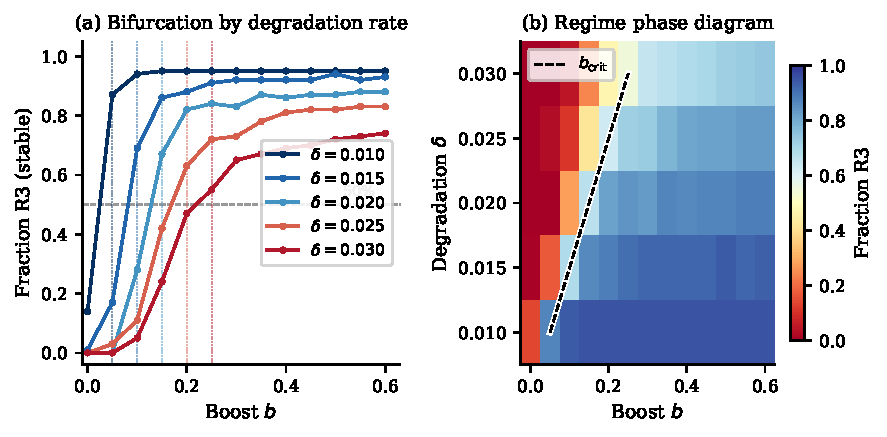
\includegraphics[width=0.70\linewidth]{fig2_regime.pdf}
\caption{Regime structure (6,500 stochastic runs). Left: R3 fraction
vs.\ boost $b$ for each $\delta$; dotted lines mark
$b_{\mathrm{crit}}(\delta)$. Right: phase diagram; blue = R3, red =
R1/R2. The $b_{\mathrm{crit}} \approx 10\delta$ scaling appears as
the diagonal boundary.}
\label{fig:regime}
\end{figure}

\subsection{Multi-modal industrial benchmark}
\label{sec:benchmark}

The 64D input is partitioned into four sensor modalities (16 dims each)
matching Example~\ref{ex:valve}. Anchor coordinates: $x_0 = 0.15,
x_{16} = 0.20, x_{32} = 0.55, x_{48} = 0.10$ (normal); $y_0 = 0.88,
y_{16} = 0.72, y_{32} = 0.22, y_{48} = 0.76$ (critical); $\Phi(z) =
\st{estop}$ iff $z_0 > 0.70$; sensor noise $\mathcal{N}(0, 0.05^2)$ on
non-anchor dims. Per-modality rates: pressure $\delta_p = 0.020$,
vibration $\delta_v = 0.015$, temperature $\delta_T = 0.012$, flow
$\delta_f = 0.007$. Pressure dominates effective degradation; temperature
and flow degrade more slowly, preserving corroborating boundary evidence
longer. Sweep: 100 seeds $\times$ 13 boost values, $T = 200$ steps,
1,300 runs total.

\begin{observation}
$b_{\mathrm{crit}} = 0.10$ in the benchmark, lower than 0.15 at uniform
$\delta = 0.020$ because slower degradation of non-pressure modalities
extends the corroborating evidence window.
\end{observation}

Benchmark recall and precision are both 100\% (right two columns of
Table~\ref{tab:conf-stoch}); mean lead time is 13.7 steps (range 7 to
24). The benchmark is not yet an adversarial benchmark: perturbations are
stochastic and modality-specific, not selected by an attacker to exhaust
enrichment. The adversarial question is therefore separated from the
empirical claim made here. Section~\ref{sec:security} identifies the
attack surface and the compound signal required for suspicion, but a
future evaluation should add a bounded probing trace that compares
$\mathcal{F}_n$ accumulation under malicious enrichment exhaustion against
the R3 stable-recovery baseline.

\begin{table}[tbp]
\centering
\caption{Cross-setting comparison of key metrics}
\label{tab:comparison}
\small
\begin{tabular}{lccc}
\toprule
\textbf{Metric} & \textbf{Deterministic} & \textbf{Stochastic} & \textbf{Benchmark} \\
 & (13 runs) & (6,500 runs) & (1,300 runs) \\
\midrule
Total runs            & 13    & 6,500   & 1,300 \\
Ruptured runs         & 8     & 1,959   & 200 \\
Recall (\st{critical}) & 100\% & 100\% & 100\% \\
Precision (\st{critical}) & 100\% & 92.9\% & 100\% \\
Mean lead time (steps) & 11.5 & 11.6 & 13.7 \\
$\mathcal{F}_n$ ratio R2/R3 & n/a & 14.9$\times$ & 13.8$\times$ \\
$b_{\mathrm{crit}}$ & 0.20 & 0.15 ($\delta$=0.020) & 0.10 \\
\bottomrule
\end{tabular}
\end{table}

\begin{observation}
Recall is 100\% in all three settings; precision varies from 92.9\%
(stochastic, where noise permits \st{critical} in runs that recover)
to 100\% (benchmark, where multi-modal degradation yields cleaner
separation).
\end{observation}

\paragraph{Reproducibility.}
All experiments were generated from the publicly available implementation
at \url{https://github.com/dhwcmoore/Structural-Fatigue-and-Metastable-Closure-in-Runtime-Monitoring};
the repository includes the OCaml state machine, stochastic sweep,
fatigue metrics, and plotting scripts required to reproduce all
reported figures and lead-time statistics.

% ── 8. Metastable Closure ─────────────────────────────────────────────────────
\section{Metastable Closure and the Recovery Principle}
\label{sec:mrp}

\begin{definition}[Metastable closure]
\label{def:metastable}
A run is \emph{metastably closed} if it achieves at least one reclosure
($\mathtt{rcls\_t} \neq -1$), subsequently ruptures
($\mathtt{rupt\_t} \neq -1$), and has positive cumulative fatigue
$\mathcal{F}_n(\mathtt{rupt\_t}) > 0$. Metastable closure corresponds
to Regime 2 in the experimental classification.
\end{definition}

A metastably closed run is not a run that almost stabilised: it
\emph{did} stabilise, appeared closed, passed any instantaneous
admissibility check, and then ruptured. R2 and R3 trajectories are
separable only by $\mathcal{F}_n$ (Table~\ref{tab:hidden}).

Let $\mathcal{E}_k$ denote episode $k$ (one \st{meta\_review}
entry-to-exit cycle), with $d_{\min}^{(k)}$ the minimum separation EMA,
$\mathcal{F}^{(k)}$ the fatigue accumulated, and $\bar{E}_r^{(k)}$ the
mean recovery elasticity during $\mathcal{E}_k$.

The following principle is model-supported, not universally proved:
the structural separation and certificate semantics are machine-checked;
the quantitative claims (i)--(iii) are empirical over the evaluated
STAK-PSAL model family.

\begin{principle}[Metastable Recovery Principle]
\label{thm:mrp}
Under the STAK-PSAL model with $\delta > 0$ and $b <
b_{\mathrm{crit}}(\delta)$, the following hold for metastably closed
runs (Definition~\ref{def:metastable}).

\textbf{Claim (i), persistent fatigue accumulation:}
$\mathbb{E}[\mathcal{F}_n \mid \mathrm{R2}] \gg
\mathbb{E}[\mathcal{F}_n \mid \mathrm{R3}]$.

\textbf{Claim (ii), elasticity depletion:}
$\min_t E_r^{(t)} < 0$ for every metastably closed run.

\textbf{Claim (iii), episode-level trend (majority):} among metastably
closed runs with $K \geq 2$ episodes, a strict majority exhibit both
$d_{\min}^{(k+1)} \leq d_{\min}^{(k)}$ and $\mathcal{F}^{(k+1)} \geq
\mathcal{F}^{(k)}$ for all $k$.

\textbf{Claim (iv), CRITICAL coverage:} no metastably closed run in any
evaluated setting terminates in \st{hard\_rupture} without having first
satisfied \eqref{eq:critical}.
\end{principle}

\begin{proof}[Empirical support]
(i) follows from Table~\ref{tab:fatigue}: R2 mean $\mathcal{F}_n = 2.462$,
R3 mean $= 0.165$, ratio $14.9\times$. (ii) follows from the same table:
$\min E_r < 0$ for 100\% of R2 runs. (iii) follows from the benchmark episode statistics:
majorities exhibit both decreasing $d_{\min}^{(k)}$ and non-decreasing
$\mathcal{F}^{(k)}$ across episodes. (iv): in 2,159 ruptured runs, none
reached \st{hard\_rupture} without first satisfying \eqref{eq:critical}.
\end{proof}

{\sloppy\paragraph{Machine-checked metastable recovery semantics.}
Three results in \texttt{formal/\allowbreak{}metastable\_recovery.v}.
(i)~\texttt{recovered\_not\_\allowbreak{}metastable}: $\mathit{recovered}(t)$
and $\mathit{metastable\_closed}(t)$ are structurally disjoint.
(ii)~\texttt{admissible\_\allowbreak{}visibility\_failure}: there exists
$t$ at which the monitor reads \st{closed} while the structural forecast
is a bounded rupture claim.
(iii)~The certificate soundness hierarchy
(\texttt{certificate\_sound},
\texttt{certificate\_\allowbreak{}within\_horizon},
\texttt{certificate\_\allowbreak{}marks\_visible\_\allowbreak{}metastability}):
a constructive rupture witness is realisable within the declared horizon
while the monitor reads \st{closed}.\par}

The empirical 13.8--14.9$\times$ fatigue ratio is not formally proved;
it is an experimental observation over the evaluated model family.

For R2 benchmark runs with $K \geq 2$ episodes ($n=190$), decreasing
$d_{\min}^{(k)}$ holds in 123 cases (65\%), non-decreasing
$\mathcal{F}^{(k)}$ in 118 cases (62\%), and decreasing
$\bar{E}_r^{(k)}$ in 72 cases (38\%). Separation and fatigue trend
conditions hold for majorities; elasticity
strict monotonicity (38\%) is weaker since episode-to-episode noise
disrupts strict ordering while the cumulative trend in claim (i)
remains clean. A status-only monitor cannot distinguish a system that
has never destabilised from one with $\mathcal{F}_n > 2$ (overwhelmingly
R2); $\mathcal{F}_n \approx 0.165$ is an empirical discriminator, not a
stability proof.

% ── 9. Security and Deployment Constraints ────────────────────────────────────
\section{Security and Deployment Constraints}
\label{sec:security}

The read-only sidecar assumption fixes the authority boundary for the adversarial analysis: an attacker may exhaust enrichment capacity through the observed system trajectory, but STAK-PSAL itself does not become an actuator.
A runtime-modifiable reduction operator introduces an attack surface
absent in immutable certified pipelines; three risk classes follow
from the enrichment structure (Section~\ref{sec:failure}).
\textit{Spoofing} of the warning condition: an adversary perturbing the
input near the safety boundary may force the monitor into
\st{meta\_review} and consume its enrichment budget, raising
$\mathcal{F}_n$ without any physical degradation, consistent with the
adversarial elasticity inversion identified in
Section~\ref{sec:estimators}.
\textit{Adversarial activation} of the enrichment pathway: a compromised
channel may inject distortions into row 0 of $W_t$ that survive the
immediate admissibility check but corrupt downstream behaviour.
\textit{Destabilisation by repeated probing}: a sequence of bounded
perturbations near the boundary can deplete the enrichment budget,
driving the system toward the R2 regime even when each individual
perturbation is benign. The attack surface is therefore not the physical process alone, but the
finite enrichment capacity of the observational boundary itself. Horizon Debt sharpens this attack surface: an adversary need not force immediate rupture, but only consume enough repair horizon that authenticated enrichment mechanisms age out before they can arrive.

Adversarial exhaustion is more dangerous than direct drive to rupture:
repeated bounded perturbations force \st{meta\_review} entry, consume
enrichment capacity, and raise $\mathcal{F}_n$ while the physical
process remains in bounds, producing adversarial elasticity inversion
(Definition~\ref{def:aei}). Negative elasticity signals intrusion only
under the compound condition of bounded $|\Delta P_t|$ and repeated
\st{meta\_review} entry; 20\% of R3 runs exhibit $\min E_r < 0$
in isolation (Table~\ref{tab:fatigue}).

Mitigation is partial and deployment-dependent. Enrichment triggers
should authenticate warning provenance; mutable pathways should be
restricted to a rate-limited API surface; immutable variants preserve the monitoring contract without
exposing the weight matrix. The security claim is deliberately bounded:
STAK-PSAL does not identify an attacker from negative elasticity alone.
It identifies a structural symptom that should not occur when the
physical degradation proxy remains bounded and the enrichment pathway is
being repeatedly exercised. A full adversarial analysis is a defined
open boundary of the present work.

% ── 10. Related Work ──────────────────────────────────────────────────────────
\section{Related Work}
\label{sec:related}

\textbf{Runtime verification and drift detection.}
Classical RV monitors traces against temporal specifications~\cite{leucker2009brief,havelund2018rule}; STAK-PSAL instead monitors the reduction operator $M_t$ to anticipate violations. Unlike conventional drift monitors evaluating current observation space, STAK-PSAL evaluates the cumulative structural cost to maintain admissibility. Predictive monitoring~\cite{zhao2021predictive,chen2009monitoring} is the closest analogue, instantiated here for admissibility degradation via $\mathcal{F}_n$.

\textbf{Monitorability and formal methods.}
The monitorability question~\cite{francalanza2017theory,bauer2011runtime} is here specialised to admissibility degradation, answering affirmatively for continuous trajectories. While static interpretation~\cite{cousot1977abstract} and CEGAR~\cite{clarke2000counterexample} establish properties pre-deployment, STAK-PSAL monitors whether the runtime reduction preserves the requisite distinctions.

\textbf{Cyber-physical systems and PHM.}
Runtime assurance for CPS~\cite{seshia2015towards,schierman2015runtime} is extended to the observation layer. Prognostics and Health Management (PHM) tracks latent fatigue accumulation~\cite{jardine2006review,chiang2014fault}; $\mathcal{F}_n$ specialises this to observational admissibility.

% ── 11. Applicability and Domain Boundaries ───────────────────────────────────
\section{Applicability, Limitations, and Domain Boundaries}
\label{sec:limits}

\textbf{Model scope and statistical claims.} The current prototype uses
a linear-nonlinear reduction with two critical vectors and scalar
degradation; multiple concurrent critical pairs $(x_i, y_i)$ are the
immediate scaling challenge, requiring fatigue aggregation or per-pair
tracking. Results are point estimates on a fixed model with calibrated
thresholds and require confidence quantification. The \st{critical}
thresholds were set on the 13 deterministic runs of
Section~\ref{sec:det-sweep}; the stochastic and benchmark sweeps are
out-of-calibration evaluations, not cross-validation. The
zero-false-negative claim is model-specific. Rapid degradation is no longer merely a reduced-lead-time limitation. It is represented by Horizon Debt: a state in which admissibility may still hold instantaneously, but timely admissibility has failed because the remaining rupture horizon is no greater than the monitor's lag. If no certified enrichment mechanism remains viable, the monitor cannot certify enrichment-mediated recovery. This does not prove physical inevitability of rupture; it proves only that recovery is no longer certified under the current mechanism catalogue and gain contracts.

\textbf{Proof and runtime gap.} The Coq theorems use
Definition~\ref{def:admissibility} (exact equality); the OCaml monitor
uses Definition~\ref{def:eps}. The threshold-crossing bridge is
machine-checked in \texttt{formal/\allowbreak{}threshold\_bridge.v} in its
existential form: under geometric contraction, crossing from any
$\varepsilon$ to any smaller $\varepsilon'$ is guaranteed in bounded
steps. Closing the remaining gap formally requires restating the
structural invariants (T1)--(T5) over Definition~\ref{def:eps}; the
explicit logarithmic ceiling bound of Lemma~\ref{lem:opbound} remains a
quantitative refinement of the mechanised existential.

\textbf{Domain boundary: continuous fatigue mathematics and discrete
generative systems.} STAK-PSAL rests on assumptions fitting continuous
degradation: multiplicative weight decay, a smooth separation margin,
an additive enrichment response, and a continuous fatigue functional.
These hold for cyber-physical processes; transfer to discrete generative
systems (LLM agents and similar) is not clean: token-level policies do
not exhibit multiplicative weight decay, the embedding analogue of
separation margin is not continuous along a trajectory, and the
operational meaning of enrichment is undefined. A possible analogue of
enrichment would be adaptive resampling, tool-mediated verification,
temperature reduction, or retrieval expansion after a warning signal; but
none of these is a direct counterpart of restoring a physical separation
margin. Applicability to discrete generative systems is therefore not an
extension claimed here. It is a separate research problem: first define a
monitorable discrete margin, then define what counts as finite recovery
elasticity for that margin.

STAK-PSAL does not prove inevitability of rupture. The monitor predicts
bounded rupture horizon under continued degradation dynamics within the
evaluated model family. Sufficient external enrichment, operator
intervention, or structural modification may still restore admissibility
before collapse.

% ── Conclusion ────────────────────────────────────────────────────────────────
\section*{Conclusion}

A runtime system may remain operationally closed while already
possessing a bounded rupture horizon. The machine-checked semantic
hierarchy (\texttt{formal/\allowbreak{}metastable\_recovery.v}) formalises this as
the admissible visibility failure theorem: operational closure does not
entail structural safety, and metastable closure admits constructive
rupture witnesses bounded within a declared horizon. The machine-checked
existential bridge (\texttt{formal/\allowbreak{}threshold\_bridge.v}) connects the
strict-equality formal layer to the $\varepsilon$-admissible operational
layer, guaranteeing threshold crossing under geometric contraction;
the explicit logarithmic ceiling bound of Lemma~\ref{lem:opbound}
is the quantitative refinement isolating the precise horizon.
STAK-PSAL operationalises these results: $\mathcal{F}_n$ tracks
cumulative structural degradation invisible to instantaneous monitors,
with \st{critical} signals providing mean lead time 11.6 to 13.7 steps
and zero false negatives in the 2,159 evaluated ruptured runs; and the
three-witness certificate emits a bounded rupture witness on confirmed
collapse. The Metastable Recovery Principle identifies the risk static
and output-level monitors cannot detect: $\mathcal{F}_n$ is
13.8--14.9$\times$ higher in metastably closed runs. Runtime assurance is therefore path-dependent rather than purely
state-dependent: admissibility may hold at time \(t\) while the history
required to preserve it still carries a bounded rupture horizon. Safety-relevant distinguishability must therefore be monitored as a
runtime quantity. STAK-PSAL therefore separates three conditions that ordinary runtime status collapses: present admissibility, timely admissibility, and durable recovery. Structural fatigue records the historical cost of remaining admissible; Horizon Debt records the moment at which admissibility remains extensionally visible but operationally too late.

% ── References ────────────────────────────────────────────────────────────────
\bibliographystyle{splncs04}

{\small
\begin{thebibliography}{99}

\bibitem{leucker2009brief}
M.~Leucker and C.~Schallhart.
A brief account of runtime verification.
\textit{Journal of Logic and Algebraic Programming}, 78(5):293--303, 2009.

\bibitem{havelund2018rule}
K.~Havelund and D.~Peled.
Runtime verification: From propositional to first-order temporal logic.
In \textit{International Conference on Runtime Verification}, pages 90--112.
Springer, 2018.

\bibitem{seshia2018verified}
S.~A.~Seshia, D.~Sadigh, and A.~D.~Dragan.
Toward verified artificial intelligence.
\textit{Communications of the ACM}, 61(7):46--55, 2018.

\bibitem{chen2009monitoring}
F.~Chen and G.~Ro\c{s}u.
Parametric trace slicing and monitoring.
In \textit{TACAS}, pages 246--261. Springer, 2009.

\bibitem{zhao2021predictive}
M.~Zhao and G.~Rozier.
Predictive runtime monitoring for linear stochastic systems.
In \textit{International Conference on Runtime Verification}, pages 382--400.
Springer, 2021.

\bibitem{kim2022fault}
E.~Kim, M.~Guo, and B.~Fidan.
Online fault prognosis for cyber-physical systems.
\textit{IEEE Transactions on Automation Science and Engineering}, 2022.

\bibitem{tuncali2018simulation}
C.~E.~Tuncali, T.~P.~Pavlic, and G.~Fainekos.
Simulation-based adversarial test generation for autonomous vehicles.
In \textit{IEEE Intelligent Vehicles Symposium}, 2018.

\bibitem{amodei2016concrete}
D.~Amodei, C.~Olah, J.~Steinhardt, P.~Christiano, J.~Schulman,
and D.~Man{\'e}.
Concrete problems in AI safety.
\textit{arXiv:1606.06565}, 2016.

\bibitem{scheffer2009early}
M.~Scheffer \textit{et al.}
Early-warning signals for critical transitions.
\textit{Nature}, 461(7260):53--59, 2009.

\bibitem{holling1973resilience}
C.~S.~Holling.
Resilience and stability of ecological systems.
\textit{Annual Review of Ecology and Systematics}, 4(1):1--23, 1973.

\bibitem{pimm1984complexity}
S.~L.~Pimm.
The complexity and stability of ecosystems.
\textit{Nature}, 307(5949):321--326, 1984.

\bibitem{cousot1977abstract}
P.~Cousot and R.~Cousot.
Abstract interpretation: A unified lattice model.
In \textit{POPL}, pages 238--252, 1977.

\bibitem{clarke2000counterexample}
E.~Clarke \textit{et al.}
Counterexample-guided abstraction refinement.
In \textit{CAV}, pages 154--169. Springer, 2000.

\bibitem{pnueli1977temporal}
A.~Pnueli.
The temporal logic of programs.
In \textit{FOCS}, pages 46--57. IEEE, 1977.

\bibitem{francalanza2017theory}
A.~Francalanza, J.~A.~P{\'e}rez, and C.~S{\'a}nchez.
Runtime verification for decentralised and distributed systems.
In \textit{Lectures on Runtime Verification}, pages 176--210. Springer, 2018.

\bibitem{bauer2011runtime}
A.~Bauer, M.~Leucker, and C.~Schallhart.
The good, the bad, and the ugly, but how ugly is ugly?
In \textit{International Conference on Runtime Verification}, pages 126--138. Springer, 2011.

\bibitem{falcone2010predictive}
Y.~Falcone, J.~J.~Hadjadj-Aoul, and T.~Jéron.
More lessons on test generation for temporal properties.
In \textit{International Workshop on Formal Methods for Testing},
pages 126--145. Springer, 2010.

\bibitem{lee2008cyber}
E.~A.~Lee and S.~A.~Seshia.
\textit{Introduction to Embedded Systems: A Cyber-Physical Systems Approach}.
MIT Press, second edition, 2017.

\bibitem{seshia2015towards}
S.~A.~Seshia and S.~Jha.
Adaptive runtime monitoring for autonomous cyber-physical systems.
In \textit{17th International Conference on Hybrid Systems: Computation and
Control}, pages 173--182. ACM, 2014.

\bibitem{viswanathan1994monitoring}
M.~Viswanathan and R.~Vardi.
Revisiting the hierarchy of until and since.
In \textit{Logic in Computer Science (LICS)}, pages 70--79. IEEE, 1994.

\bibitem{saxe2010statistical}
A.~M.~Saxe, Y.~Barda, and T.~B.~Bright.
Mitigating adversarial effects through randomization.
In \textit{International Conference on Learning Representations}, 2019.

\bibitem{pham2016phm}
H.~T.~Pham, A.~Khatkhate, Y.~Zhang, and Z.~Gao.
Probabilistic approach to remaining useful life estimation.
\textit{Annual Reviews in Control}, 39:133--142, 2015.

\bibitem{li2018degradation}
Y.~Li, N.~Chen, J.~Xu, and X.~Sheng.
Degradation data analysis based on a wiener process with
multiple change-points and measurement error.
\textit{European Journal of Operational Research}, 271(2):641--652, 2018.

\bibitem{chiang2014fault}
L.~H.~Chiang, E.~L.~Russell, and R.~D.~Braatz.
\textit{Fault Detection and Diagnosis in Industrial Systems}.
Springer Science+Business Media, 2001.

\bibitem{schierman2015runtime}
J.~D.~Schierman, D.~G.~Ward, N.~D.~Richards, N.~Gandhi, J.~F.~Hammer,
and D.~B.~Murray.
Runtime assurance for advanced flight-critical systems.
\textit{IEEE Transactions on Aerospace and Electronic Systems},
51(4):2931--2945, 2015.

\bibitem{jardine2006review}
A.~K.~S.~Jardine, D.~Lin, and D.~Banjevic.
A review on machinery diagnostics and prognostics implementing
condition-based maintenance.
\textit{Mechanical Systems and Signal Processing}, 20(7):1483--1510, 2006.

\end{thebibliography}
}

\end{document}
